% Options for packages loaded elsewhere
\PassOptionsToPackage{unicode}{hyperref}
\PassOptionsToPackage{hyphens}{url}
\PassOptionsToPackage{dvipsnames,svgnames*,x11names*}{xcolor}
%
\documentclass[
]{article}
\usepackage{lmodern}
\usepackage{amssymb,amsmath}
\usepackage{ifxetex,ifluatex}
\ifnum 0\ifxetex 1\fi\ifluatex 1\fi=0 % if pdftex
  \usepackage[T1]{fontenc}
  \usepackage[utf8]{inputenc}
  \usepackage{textcomp} % provide euro and other symbols
\else % if luatex or xetex
  \usepackage{unicode-math}
  \defaultfontfeatures{Scale=MatchLowercase}
  \defaultfontfeatures[\rmfamily]{Ligatures=TeX,Scale=1}
  \setmainfont[]{cochineal}
  \setsansfont[]{Fira Sans}
  \setmonofont[]{Fira Code}
\fi
% Use upquote if available, for straight quotes in verbatim environments
\IfFileExists{upquote.sty}{\usepackage{upquote}}{}
\IfFileExists{microtype.sty}{% use microtype if available
  \usepackage[]{microtype}
  \UseMicrotypeSet[protrusion]{basicmath} % disable protrusion for tt fonts
}{}
\makeatletter
\@ifundefined{KOMAClassName}{% if non-KOMA class
  \IfFileExists{parskip.sty}{%
    \usepackage{parskip}
  }{% else
    \setlength{\parindent}{0pt}
    \setlength{\parskip}{6pt plus 2pt minus 1pt}}
}{% if KOMA class
  \KOMAoptions{parskip=half}}
\makeatother
\usepackage{xcolor}
\IfFileExists{xurl.sty}{\usepackage{xurl}}{} % add URL line breaks if available
\IfFileExists{bookmark.sty}{\usepackage{bookmark}}{\usepackage{hyperref}}
\hypersetup{
  pdftitle={Data Science for Economists},
  colorlinks=true,
  linkcolor=Maroon,
  filecolor=Maroon,
  citecolor=Blue,
  urlcolor=blue,
  pdfcreator={LaTeX via pandoc}}
\urlstyle{same} % disable monospaced font for URLs
\usepackage[margin=1in]{geometry}
\usepackage{color}
\usepackage{fancyvrb}
\newcommand{\VerbBar}{|}
\newcommand{\VERB}{\Verb[commandchars=\\\{\}]}
\DefineVerbatimEnvironment{Highlighting}{Verbatim}{commandchars=\\\{\}}
% Add ',fontsize=\small' for more characters per line
\usepackage{framed}
\definecolor{shadecolor}{RGB}{248,248,248}
\newenvironment{Shaded}{\begin{snugshade}}{\end{snugshade}}
\newcommand{\AlertTok}[1]{\textcolor[rgb]{0.94,0.16,0.16}{#1}}
\newcommand{\AnnotationTok}[1]{\textcolor[rgb]{0.56,0.35,0.01}{\textbf{\textit{#1}}}}
\newcommand{\AttributeTok}[1]{\textcolor[rgb]{0.13,0.29,0.53}{#1}}
\newcommand{\BaseNTok}[1]{\textcolor[rgb]{0.00,0.00,0.81}{#1}}
\newcommand{\BuiltInTok}[1]{#1}
\newcommand{\CharTok}[1]{\textcolor[rgb]{0.31,0.60,0.02}{#1}}
\newcommand{\CommentTok}[1]{\textcolor[rgb]{0.56,0.35,0.01}{\textit{#1}}}
\newcommand{\CommentVarTok}[1]{\textcolor[rgb]{0.56,0.35,0.01}{\textbf{\textit{#1}}}}
\newcommand{\ConstantTok}[1]{\textcolor[rgb]{0.56,0.35,0.01}{#1}}
\newcommand{\ControlFlowTok}[1]{\textcolor[rgb]{0.13,0.29,0.53}{\textbf{#1}}}
\newcommand{\DataTypeTok}[1]{\textcolor[rgb]{0.13,0.29,0.53}{#1}}
\newcommand{\DecValTok}[1]{\textcolor[rgb]{0.00,0.00,0.81}{#1}}
\newcommand{\DocumentationTok}[1]{\textcolor[rgb]{0.56,0.35,0.01}{\textbf{\textit{#1}}}}
\newcommand{\ErrorTok}[1]{\textcolor[rgb]{0.64,0.00,0.00}{\textbf{#1}}}
\newcommand{\ExtensionTok}[1]{#1}
\newcommand{\FloatTok}[1]{\textcolor[rgb]{0.00,0.00,0.81}{#1}}
\newcommand{\FunctionTok}[1]{\textcolor[rgb]{0.13,0.29,0.53}{\textbf{#1}}}
\newcommand{\ImportTok}[1]{#1}
\newcommand{\InformationTok}[1]{\textcolor[rgb]{0.56,0.35,0.01}{\textbf{\textit{#1}}}}
\newcommand{\KeywordTok}[1]{\textcolor[rgb]{0.13,0.29,0.53}{\textbf{#1}}}
\newcommand{\NormalTok}[1]{#1}
\newcommand{\OperatorTok}[1]{\textcolor[rgb]{0.81,0.36,0.00}{\textbf{#1}}}
\newcommand{\OtherTok}[1]{\textcolor[rgb]{0.56,0.35,0.01}{#1}}
\newcommand{\PreprocessorTok}[1]{\textcolor[rgb]{0.56,0.35,0.01}{\textit{#1}}}
\newcommand{\RegionMarkerTok}[1]{#1}
\newcommand{\SpecialCharTok}[1]{\textcolor[rgb]{0.81,0.36,0.00}{\textbf{#1}}}
\newcommand{\SpecialStringTok}[1]{\textcolor[rgb]{0.31,0.60,0.02}{#1}}
\newcommand{\StringTok}[1]{\textcolor[rgb]{0.31,0.60,0.02}{#1}}
\newcommand{\VariableTok}[1]{\textcolor[rgb]{0.00,0.00,0.00}{#1}}
\newcommand{\VerbatimStringTok}[1]{\textcolor[rgb]{0.31,0.60,0.02}{#1}}
\newcommand{\WarningTok}[1]{\textcolor[rgb]{0.56,0.35,0.01}{\textbf{\textit{#1}}}}
\usepackage{longtable,booktabs}
% Correct order of tables after \paragraph or \subparagraph
\usepackage{etoolbox}
\makeatletter
\patchcmd\longtable{\par}{\if@noskipsec\mbox{}\fi\par}{}{}
\makeatother
% Allow footnotes in longtable head/foot
\IfFileExists{footnotehyper.sty}{\usepackage{footnotehyper}}{\usepackage{footnote}}
\makesavenoteenv{longtable}
\usepackage{graphicx}
\makeatletter
\def\maxwidth{\ifdim\Gin@nat@width>\linewidth\linewidth\else\Gin@nat@width\fi}
\def\maxheight{\ifdim\Gin@nat@height>\textheight\textheight\else\Gin@nat@height\fi}
\makeatother
% Scale images if necessary, so that they will not overflow the page
% margins by default, and it is still possible to overwrite the defaults
% using explicit options in \includegraphics[width, height, ...]{}
\setkeys{Gin}{width=\maxwidth,height=\maxheight,keepaspectratio}
% Set default figure placement to htbp
\makeatletter
\def\fps@figure{htbp}
\makeatother
\setlength{\emergencystretch}{3em} % prevent overfull lines
\providecommand{\tightlist}{%
  \setlength{\itemsep}{0pt}\setlength{\parskip}{0pt}}
\setcounter{secnumdepth}{-\maxdimen} % remove section numbering
%% See: https://bookdown.org/yihui/rmarkdown-cookbook/multi-column.html
%% I've made some additional adjustments based on my own preferences (e.g. cols
%% should be top-aligned in case of uneven vertical length)
\newenvironment{columns}[1][]{}{}

\newenvironment{column}[1]{\begin{minipage}[t]{#1}\ignorespaces}{%
\end{minipage}
\ifhmode\unskip\fi
\aftergroup\useignorespacesandallpars
}

\def\useignorespacesandallpars#1\ignorespaces\fi{%
#1\fi\ignorespacesandallpars}

\makeatletter
\def\ignorespacesandallpars{%
  \@ifnextchar\par
    {\expandafter\ignorespacesandallpars\@gobble}%
    {}%
}
\makeatother

\title{Data Science for Economists}
\usepackage{etoolbox}
\makeatletter
\providecommand{\subtitle}[1]{% add subtitle to \maketitle
  \apptocmd{\@title}{\par {\large #1 \par}}{}{}
}
\makeatother
\subtitle{Lecture 16: Databases}
\usepackage{authblk}
                                        \author[]{Grant R. McDermott}
                                                            \affil{University
of Oregon \textbar{} \href{https://github.com/uo-ec607/lectures}{EC
607}}
                                            \date{}

\begin{document}
\maketitle

{
\hypersetup{linkcolor=}
\setcounter{tocdepth}{2}
\tableofcontents
}
\hypertarget{requirements}{%
\subsection{Requirements}\label{requirements}}

\hypertarget{create-an-account-on-google-cloud-platform-free}{%
\subsubsection{Create an account on Google Cloud Platform
(free)}\label{create-an-account-on-google-cloud-platform-free}}

You should already have done this for the lecture on Google Compute
Engine. See
\href{https://raw.githack.com/uo-ec607/lectures/master/14-gce-i/14-gce-i.html\#Create_an_account_on_Google_Cloud_Platform_(free)}{here}
if not.

\hypertarget{r-packages}{%
\subsubsection{R packages}\label{r-packages}}

\begin{itemize}
\tightlist
\item
  New: \textbf{DBI}, \textbf{duckdb}, \textbf{bigrquery}, \textbf{glue}
\item
  Already used: \textbf{tidyverse}, \textbf{hrbrthemes},
  \textbf{nycflights13}
\end{itemize}

As per usual, the code chunk below will install (if necessary) and load
all of these packages for you. I'm also going to set my preferred
ggplot2 theme, but as you wish.

\begin{Shaded}
\begin{Highlighting}[]
\DocumentationTok{\#\# Load/install packages}
\ControlFlowTok{if}\NormalTok{ (}\SpecialCharTok{!}\FunctionTok{require}\NormalTok{(}\StringTok{"pacman"}\NormalTok{)) }\FunctionTok{install.packages}\NormalTok{(}\StringTok{"pacman"}\NormalTok{)}
\NormalTok{pacman}\SpecialCharTok{::}\FunctionTok{p\_load}\NormalTok{(tidyverse, DBI, duckdb, bigrquery, hrbrthemes, nycflights13, glue)}
\DocumentationTok{\#\# My preferred ggplot2 theme (optional)}
\FunctionTok{theme\_set}\NormalTok{(hrbrthemes}\SpecialCharTok{::}\FunctionTok{theme\_ipsum}\NormalTok{())}
\end{Highlighting}
\end{Shaded}

\hypertarget{databases-101}{%
\subsection{Databases 101}\label{databases-101}}

Many ``big data'' problems could be more accurately described as ``small
data problems in disguise''. Which is to say, the data that we care
about is only a subset or aggregation of some larger dataset. For
example, we might want to access US Census data\ldots{} but only for a
handful of counties along the border of two contiguous states. Or, we
might want to analyse climate data collected from a large number of
weather stations\ldots{} but aggregated up to the national or monthly
level. In such cases, the underlying bottleneck is interacting with the
original data, which is too big to fit into memory. How do we store data
of this magnitude and and then access it effectively? The answer is
through a \textbf{database}.

Databases can exist either locally or remotely, as well as in-memory or
on-disk. Regardless of where a database is located, the key point is
that information is stored in a way that allows for very quick
extraction and/or aggregation. Think back to our filing cabinet analogy
from the \textbf{data.table} lecture:

\begin{quote}
A filing cabinet arranges items by alphabetical order: Files starting
``ABC'' in the top drawer, ``DEF'' in the second drawer, etc. To find
Alice's file, you'd only have to search the top draw. For Fred, the
second draw, and so on.
\end{quote}

This analogy, whilst slightly imperfect, captures the essence of what
makes databases so efficient.\footnote{In truth, most databases rely on
  \href{https://en.wikipedia.org/wiki/Binary_search_tree}{binary search
  trees} (``b-trees''). A b-tree shares the spirit of the file cabinet
  ordering system, but takes it step further so that we eliminate at
  least half of the remaining data from our search at each step. E.g. We
  need to find a person's tax records in a million-row dataset. In the
  first step we immediately realise that it's somewhere in the first
  500k rows. In the next step we immediately realise that it's somewhere
  in rows 250k-500k, etc.} They can very quickly identify the components
that they need to focus on for a particular operation. Extracting the
specific information that we want is a simple matter of submitting a
\textbf{query} to the database. The query is where we tell the database
how to manipulate or subset the data into a more manageable form, which
we can then pull into our analysis environment (R, Python, etc.)

At this point, you might be tempted to think of a database as the
``thing'' that you interact with directly. However, it's important to
realise that the data are actually organised in one or more
\textbf{tables} within the database. These tables are rectangular,
consisting of rows and columns, where each row is identified by a unique
key. In that sense, they are very much like the data frames that we're
all used to working with. Continuing with the analogy, a database then
is rather like a list of data frames of R. To access information from a
specific table (data frame), we first have to index it from the database
(list) and then execute our query functions. The only material
difference being that databases can hold much more information and are
extremely efficient at executing queries over their vast contents.

\begin{quote}
\textbf{Tip:} A table in a database is like a data frame in an R list.
\end{quote}

\hypertarget{databases-and-r}{%
\subsection{Databases and R}\label{databases-and-r}}

Virtually every database in existence makes use of
\href{https://en.wikipedia.org/wiki/SQL}{\textbf{SQL}}
(\textbf{S}tructured \textbf{Q}uery \textbf{L}anguage ). SQL is an
extremely powerful tool and has become something of prerequisite for
many data science jobs.
(\href{https://raw.githack.com/uo-ec607/lectures/master/01-intro/01-Intro.html\#whyr}{Exhibit
A}.) However, it is also an archaic language that is much less intuitive
than the R tools that we have using thus far in the course. We'll see
several examples of this shortly, but first the good news: You already
have all the programming skills you need to start working with
databases. This is because the tidyverse --- through \textbf{dplyr} ---
allows for direct communication with databases from your local R
environment.

What does this mean?

Simply that you can interact with the vast datasets that are stored in
relational databases using the \emph{same} tidyverse verbs and syntax
that we already know. All of this is possible thanks to the
\textbf{dbplyr} package (\href{https://dbplyr.tidyverse.org/}{link}),
which provides a database backend to \textbf{dplyr}. What's happening
even further behind the scenes is that, upon installation,
\textbf{dbplyr} suggests the \textbf{DBI} package
(\href{https://db.rstudio.com/dbi}{link}) as a dependency. \textbf{DBI}
provides a common interface that allows \textbf{dplyr} to work with many
different databases using exactly the same code. You don't even need to
leave your RStudio session or learn SQL!

\begin{quote}
\textbf{Aside:} Okay, you will probably want to learn SQL eventually.
Luckily, \textbf{dplyr} and \textbf{dbplyr} come with several features
that can really help to speed up the learning and translation process.
We'll get to these later in the lecture.
\end{quote}

While \textbf{DBI} is automatically bundled with \textbf{dbplyr}, you'll
need to install a specific backend package for the type of database that
you want to connect to. You can see a list of commonly used backends
\href{https://db.rstudio.com/dplyr/\#getting-started}{here}. For today,
however, we'll focus on two:

\begin{enumerate}
\def\labelenumi{\arabic{enumi}.}
\tightlist
\item
  \textbf{duckdb} embeds a DuckDB database.
\item
  \textbf{bigrquery} connects to Google BigQuery.
\end{enumerate}

The former is a lightweight --- but extremely powerful ---
\href{https://en.wikipedia.org/wiki/Database\#Database_management_system}{database
management system (DBMS)} that can exist on our local computers. It thus
provides the simplest way of demonstrating the key concepts of this
section without the additional overhead required by some other common
other DBMSs. (No external dependencies, no need to connect to a remote
server, etc.) The latter is the one that I use most frequently in my own
work and also requires minimal overhead, seeing as we already set up a
Google Cloud account in the previous lecture.

\hypertarget{getting-started-duckdb}{%
\subsection{Getting started: DuckDB}\label{getting-started-duckdb}}

Our goal for this section is to create a makeshift database on our local
computers --- using the excellent
\href{https://duckdb.org/docs/api/r}{DuckDB} backend --- and then
connect to it from R. I'll use this to demonstrate the ease with which
we can execute queries from R, as well as underscore some principles for
working with databases in general. The lessons that we learn here will
carry over to more complicated cases and much larger datasets.

\hypertarget{connecting-to-a-database}{%
\subsubsection{Connecting to a
database}\label{connecting-to-a-database}}

Start by opening an (empty) database connection via the
\texttt{DBI::dbConnect()} function, which we'll call \texttt{con}. Note
that we are calling the \textbf{duckdb} package in the background for
the DuckDB backend and telling R that this is a local connection that
exists in memory.

\begin{Shaded}
\begin{Highlighting}[]
\CommentTok{\# library(DBI) \#\# Already loaded}

\NormalTok{con }\OtherTok{=} \FunctionTok{dbConnect}\NormalTok{(duckdb}\SpecialCharTok{::}\FunctionTok{duckdb}\NormalTok{(), }\AttributeTok{path =} \StringTok{":memory:"}\NormalTok{)}
\end{Highlighting}
\end{Shaded}

The arguments to \texttt{DBI::dbConnect()} vary from database to
database. However, the first argument is always the database backend,
i.e.~\texttt{duckdb::duckdb()} in this case since we're using DuckDB.
Again, while this differs depending on the database type that you're
connecting with, DuckDB only needs one other argument: the \texttt{path}
to the database. Here we use the special string, ``:memory:'', which
causes DuckDB to make a temporary in-memory database. We'll explore more
complicated connections later on that will involve things like password
prompts for remote databases.

Our makeshift database connection \texttt{con} is currently empty. So
let's copy across the \emph{flights} dataset that comes bundled together
with the \textbf{nycflights13} package. There are a couple of ways to do
this, but here I'll use the \texttt{dplyr::copy\_to()} convenience
function. Note that we are specifying the table name (``flights'') that
will exist within this database. You can also see that we're passing a
list of indexes to the \texttt{copy\_to()} function. Indexes are what
enable efficient database performance, since they specify how the data
should be laid out for very quick search and aggregation.\footnote{Again,
  dDatabases rely on
  \href{https://en.wikipedia.org/wiki/Binary_search_algorithm}{binary
  search}, which is the same algorithmic approach that we used when we
  \href{https://raw.githack.com/uo-ec607/lectures/master/05-datatable/05-datatable.html\#keys}{set
  keys} back in the \textbf{data.table} lecture.} At the same time, I
don't want you to worry too much about this right now. Indexes will be
set by the database host platform or maintainer in normal applications.

\begin{Shaded}
\begin{Highlighting}[]
\CommentTok{\# library(dplyr)        \#\# Already loaded}
\CommentTok{\# library(nycflights13) \#\# Already loaded}

\FunctionTok{copy\_to}\NormalTok{(}
  \AttributeTok{dest =}\NormalTok{ con, }
  \AttributeTok{df =}\NormalTok{ nycflights13}\SpecialCharTok{::}\NormalTok{flights, }
  \AttributeTok{name =} \StringTok{"flights"}\NormalTok{,}
  \AttributeTok{temporary =} \ConstantTok{FALSE}\NormalTok{, }
  \AttributeTok{indexes =} \FunctionTok{list}\NormalTok{(}
    \FunctionTok{c}\NormalTok{(}\StringTok{"year"}\NormalTok{, }\StringTok{"month"}\NormalTok{, }\StringTok{"day"}\NormalTok{), }
    \StringTok{"carrier"}\NormalTok{, }
    \StringTok{"tailnum"}\NormalTok{,}
    \StringTok{"dest"}
\NormalTok{    )}
\NormalTok{  )}
\end{Highlighting}
\end{Shaded}

Now that we've copied over the data, we can reference it from R via the
\texttt{dplyr::tbl()} function. This will allow us to treat it as a
normal data frame that be manipulated with \textbf{dplyr} commands.

\begin{Shaded}
\begin{Highlighting}[]
\DocumentationTok{\#\# List tables in our DuckDB database connection (optional)}
\CommentTok{\# dbListTables(con)}

\DocumentationTok{\#\# Reference the table from R}
\NormalTok{flights\_db }\OtherTok{=} \FunctionTok{tbl}\NormalTok{(con, }\StringTok{"flights"}\NormalTok{)}
\NormalTok{flights\_db}
\end{Highlighting}
\end{Shaded}

\begin{verbatim}
## # Source:   table<flights> [?? x 19]
## # Database: DuckDB 0.8.1 [Lukas@Windows 10 x64:R 4.2.2/:memory:]
##     year month   day dep_time sched_de~1 dep_d~2 arr_t~3 sched~4 arr_d~5 carrier
##    <int> <int> <int>    <int>      <int>   <dbl>   <int>   <int>   <dbl> <chr>  
##  1  2013     1     1      517        515       2     830     819      11 UA     
##  2  2013     1     1      533        529       4     850     830      20 UA     
##  3  2013     1     1      542        540       2     923     850      33 AA     
##  4  2013     1     1      544        545      -1    1004    1022     -18 B6     
##  5  2013     1     1      554        600      -6     812     837     -25 DL     
##  6  2013     1     1      554        558      -4     740     728      12 UA     
##  7  2013     1     1      555        600      -5     913     854      19 B6     
##  8  2013     1     1      557        600      -3     709     723     -14 EV     
##  9  2013     1     1      557        600      -3     838     846      -8 B6     
## 10  2013     1     1      558        600      -2     753     745       8 AA     
## # ... with more rows, 9 more variables: flight <int>, tailnum <chr>,
## #   origin <chr>, dest <chr>, air_time <dbl>, distance <dbl>, hour <dbl>,
## #   minute <dbl>, time_hour <dttm>, and abbreviated variable names
## #   1: sched_dep_time, 2: dep_delay, 3: arr_time, 4: sched_arr_time,
## #   5: arr_delay
\end{verbatim}

It worked! Everything looks pretty good, although you may notice
something slightly strange about the output. We'll get to that in a
minute.

\hypertarget{generating-queries}{%
\subsubsection{Generating queries}\label{generating-queries}}

Again, one of the best things about \textbf{dplyr} is that it
automatically translates tidyverse-style code into SQL for you. In fact,
many of the key \textbf{dplyr} verbs are based on SQL equivalents. With
that in mind, let's try out a few queries using the typical
\textbf{dplyr} syntax that we already know.

\begin{Shaded}
\begin{Highlighting}[]
\DocumentationTok{\#\# Select some columns}
\NormalTok{flights\_db }\SpecialCharTok{\%\textgreater{}\%} \FunctionTok{select}\NormalTok{(year}\SpecialCharTok{:}\NormalTok{day, dep\_delay, arr\_delay)}
\end{Highlighting}
\end{Shaded}

\begin{verbatim}
## # Source:   SQL [?? x 5]
## # Database: DuckDB 0.8.1 [Lukas@Windows 10 x64:R 4.2.2/:memory:]
##     year month   day dep_delay arr_delay
##    <int> <int> <int>     <dbl>     <dbl>
##  1  2013     1     1         2        11
##  2  2013     1     1         4        20
##  3  2013     1     1         2        33
##  4  2013     1     1        -1       -18
##  5  2013     1     1        -6       -25
##  6  2013     1     1        -4        12
##  7  2013     1     1        -5        19
##  8  2013     1     1        -3       -14
##  9  2013     1     1        -3        -8
## 10  2013     1     1        -2         8
## # ... with more rows
\end{verbatim}

\begin{Shaded}
\begin{Highlighting}[]
\DocumentationTok{\#\# Filter according to some condition}
\NormalTok{flights\_db }\SpecialCharTok{\%\textgreater{}\%} \FunctionTok{filter}\NormalTok{(dep\_delay }\SpecialCharTok{\textgreater{}} \DecValTok{240}\NormalTok{) }
\end{Highlighting}
\end{Shaded}

\begin{verbatim}
## # Source:   SQL [?? x 19]
## # Database: DuckDB 0.8.1 [Lukas@Windows 10 x64:R 4.2.2/:memory:]
##     year month   day dep_time sched_de~1 dep_d~2 arr_t~3 sched~4 arr_d~5 carrier
##    <int> <int> <int>    <int>      <int>   <dbl>   <int>   <int>   <dbl> <chr>  
##  1  2013     1     1      848       1835     853    1001    1950     851 MQ     
##  2  2013     1     1     1815       1325     290    2120    1542     338 EV     
##  3  2013     1     1     1842       1422     260    1958    1535     263 EV     
##  4  2013     1     1     2115       1700     255    2330    1920     250 9E     
##  5  2013     1     1     2205       1720     285      46    2040     246 AA     
##  6  2013     1     1     2343       1724     379     314    1938     456 EV     
##  7  2013     1     2     1332        904     268    1616    1128     288 EV     
##  8  2013     1     2     1412        838     334    1710    1147     323 UA     
##  9  2013     1     2     1607       1030     337    2003    1355     368 AA     
## 10  2013     1     2     2131       1512     379    2340    1741     359 UA     
## # ... with more rows, 9 more variables: flight <int>, tailnum <chr>,
## #   origin <chr>, dest <chr>, air_time <dbl>, distance <dbl>, hour <dbl>,
## #   minute <dbl>, time_hour <dttm>, and abbreviated variable names
## #   1: sched_dep_time, 2: dep_delay, 3: arr_time, 4: sched_arr_time,
## #   5: arr_delay
\end{verbatim}

\begin{Shaded}
\begin{Highlighting}[]
\DocumentationTok{\#\# Get the mean delay by destination (group and then summarise)}
\NormalTok{flights\_db }\SpecialCharTok{\%\textgreater{}\%}
  \FunctionTok{group\_by}\NormalTok{(dest) }\SpecialCharTok{\%\textgreater{}\%}
  \FunctionTok{summarise}\NormalTok{(}\AttributeTok{mean\_dep\_delay =} \FunctionTok{mean}\NormalTok{(dep\_delay))}
\end{Highlighting}
\end{Shaded}

\begin{verbatim}
## Warning: Missing values are always removed in SQL aggregation functions.
## Use `na.rm = TRUE` to silence this warning
## This warning is displayed once every 8 hours.
\end{verbatim}

\begin{verbatim}
## # Source:   SQL [?? x 2]
## # Database: DuckDB 0.8.1 [Lukas@Windows 10 x64:R 4.2.2/:memory:]
##    dest  mean_dep_delay
##    <chr>          <dbl>
##  1 ATL            12.5 
##  2 ORD            13.6 
##  3 RDU            12.4 
##  4 IAD            17.0 
##  5 DTW            11.8 
##  6 LAX             9.40
##  7 MIA             8.88
##  8 MEM            15.7 
##  9 CLT             9.22
## 10 MCO            11.3 
## # ... with more rows
\end{verbatim}

Again, everything seems to be working great with the minor exception
being that our output looks a little different to normal. In particular,
you might be wondering what \texttt{\#\ Source:\ \ \ lazy\ query} means.

\hypertarget{laziness-as-a-virtue}{%
\subsubsection{Laziness as a virtue}\label{laziness-as-a-virtue}}

The \emph{modus operandi} of \textbf{dplyr} is to be as lazy as
possible. What this means in practice is that your R code is translated
into SQL and executed in the database, not in R. This is a good thing,
since:

\begin{itemize}
\tightlist
\item
  It never pulls data into R unless you explicitly ask for it.
\item
  It delays doing any work until the last possible moment: it collects
  together everything you want to do and then sends it to the database
  in one step.
\end{itemize}

For example, consider an example where we are interested in the mean
departure and arrival delays for each plane (i.e.~by unique tail
number). I'll also drop observations with less than 100 flights.

\begin{Shaded}
\begin{Highlighting}[]
\NormalTok{tailnum\_delay\_db }\OtherTok{=} 
\NormalTok{  flights\_db }\SpecialCharTok{\%\textgreater{}\%} 
  \FunctionTok{group\_by}\NormalTok{(tailnum) }\SpecialCharTok{\%\textgreater{}\%}
  \FunctionTok{summarise}\NormalTok{(}
    \AttributeTok{mean\_dep\_delay =} \FunctionTok{mean}\NormalTok{(dep\_delay),}
    \AttributeTok{mean\_arr\_delay =} \FunctionTok{mean}\NormalTok{(arr\_delay),}
    \AttributeTok{n =} \FunctionTok{n}\NormalTok{()}
\NormalTok{    ) }\SpecialCharTok{\%\textgreater{}\%}
  \FunctionTok{filter}\NormalTok{(n }\SpecialCharTok{\textgreater{}} \DecValTok{100}\NormalTok{) }\SpecialCharTok{\%\textgreater{}\%} 
  \FunctionTok{arrange}\NormalTok{(}\FunctionTok{desc}\NormalTok{(mean\_arr\_delay))}
\end{Highlighting}
\end{Shaded}

Surprisingly, this sequence of operations never touches the
database.\footnote{It's a little hard to tell from this simple example,
  but an additional clue is that fact that this sequence of commands
  would execute instantaneously even it it was applied on a massive
  remote database.} It's not until you actually ask for the data (say,
by printing \texttt{tailnum\_delay\_db}) that \textbf{dplyr} generates
the SQL and requests the results from the database. Even then it tries
to do as little work as possible and only pulls down a few rows.

\begin{Shaded}
\begin{Highlighting}[]
\NormalTok{tailnum\_delay\_db}
\end{Highlighting}
\end{Shaded}

\begin{verbatim}
## # Source:     SQL [?? x 4]
## # Database:   DuckDB 0.8.1 [Lukas@Windows 10 x64:R 4.2.2/:memory:]
## # Ordered by: desc(mean_arr_delay)
##    tailnum mean_dep_delay mean_arr_delay     n
##    <chr>            <dbl>          <dbl> <dbl>
##  1 N11119            32.6           30.3   148
##  2 N16919            32.4           29.9   251
##  3 N14998            29.4           27.9   230
##  4 N15910            29.3           27.6   280
##  5 N13123            29.6           26.0   121
##  6 N11192            27.5           25.9   154
##  7 N14950            26.2           25.3   219
##  8 N21130            27.0           25.0   126
##  9 N24128            24.8           24.9   129
## 10 N22971            26.5           24.7   230
## # ... with more rows
\end{verbatim}

\hypertarget{collect-the-data-into-your-local-r-environment}{%
\subsubsection{Collect the data into your local R
environment}\label{collect-the-data-into-your-local-r-environment}}

Typically, you'll iterate a few times before you figure out what data
you need from the database. Once you've figured it out, use
\textbf{\texttt{collect()}} to pull all the data into a local data
frame. I'm going to assign this collected data frame to a new object
(i.e.~\texttt{tailnum\_delay}), but only because I want to keep the
queried data base object (\texttt{tailnum\_delay\_db}) separate for
demonstrating some SQL translation principles in the next section.

\begin{Shaded}
\begin{Highlighting}[]
\NormalTok{tailnum\_delay }\OtherTok{=} 
\NormalTok{  tailnum\_delay\_db }\SpecialCharTok{\%\textgreater{}\%} 
  \FunctionTok{collect}\NormalTok{()}
\NormalTok{tailnum\_delay}
\end{Highlighting}
\end{Shaded}

\begin{verbatim}
## # A tibble: 1,201 x 4
##    tailnum mean_dep_delay mean_arr_delay     n
##    <chr>            <dbl>          <dbl> <dbl>
##  1 N11119            32.6           30.3   148
##  2 N16919            32.4           29.9   251
##  3 N14998            29.4           27.9   230
##  4 N15910            29.3           27.6   280
##  5 N13123            29.6           26.0   121
##  6 N11192            27.5           25.9   154
##  7 N14950            26.2           25.3   219
##  8 N21130            27.0           25.0   126
##  9 N24128            24.8           24.9   129
## 10 N22971            26.5           24.7   230
## # ... with 1,191 more rows
\end{verbatim}

Super. We have successfully pulled the queried database into our local R
environment as a data frame. You can now proceed to use it in exactly
the same way as you would any other data frame. For example, we could
plot the data to see i) whether there is a relationship between mean
departure and arrival delays (there is), and ii) whether planes manage
to make up some time if they depart late (they do).

\begin{Shaded}
\begin{Highlighting}[]
\NormalTok{tailnum\_delay }\SpecialCharTok{\%\textgreater{}\%}
  \FunctionTok{ggplot}\NormalTok{(}\FunctionTok{aes}\NormalTok{(}\AttributeTok{x=}\NormalTok{mean\_dep\_delay, }\AttributeTok{y=}\NormalTok{mean\_arr\_delay, }\AttributeTok{size=}\NormalTok{n)) }\SpecialCharTok{+}
  \FunctionTok{geom\_point}\NormalTok{(}\AttributeTok{alpha=}\FloatTok{0.3}\NormalTok{) }\SpecialCharTok{+}
  \FunctionTok{geom\_abline}\NormalTok{(}\AttributeTok{intercept =} \DecValTok{0}\NormalTok{, }\AttributeTok{slope =} \DecValTok{1}\NormalTok{, }\AttributeTok{col=}\StringTok{"orange"}\NormalTok{) }\SpecialCharTok{+}
  \FunctionTok{coord\_fixed}\NormalTok{()}
\end{Highlighting}
\end{Shaded}

\begin{verbatim}
## Warning: Removed 1 rows containing missing values (`geom_point()`).
\end{verbatim}

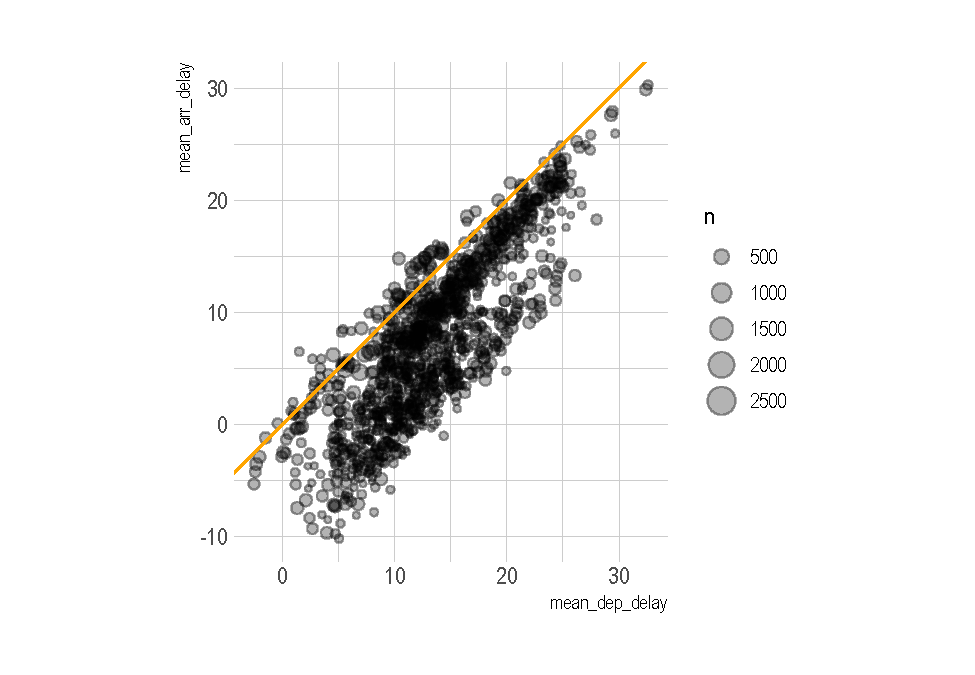
\includegraphics{16-databases_files/figure-latex/tailnum_delay_ggplot-1.pdf}

\hypertarget{joins}{%
\subsubsection{Joins}\label{joins}}

One of the things that databases excel at are joins. At interesting
touchpoint here is that \textbf{dplyr}'s collection of joining functions
are based on their SQL equivalents (including names). You'll hence be
relieved to know that the translation carries over rather nicely for
joins too. Here is a simple example, using the exact same left join that
\href{https://raw.githack.com/uo-ec607/lectures/master/05-tidyverse/05-tidyverse.html\#joins}{we
saw} back in the \textbf{tidyverse} lecture. Note that I'm copying over
the \texttt{planes} data frame to the same DuckDB connection that is
housing the \texttt{flights} table. Again, I want to emphasise that
databases are like lists, in the sense that they can hold multiple
datasets (i.e.~tables).

\begin{Shaded}
\begin{Highlighting}[]
\DocumentationTok{\#\# Copy over the "planes" dataset to the same "con" DuckDB connection.}
\FunctionTok{copy\_to}\NormalTok{(}
    \AttributeTok{dest =}\NormalTok{ con, }
    \AttributeTok{df =}\NormalTok{ nycflights13}\SpecialCharTok{::}\NormalTok{planes, }
    \AttributeTok{name =} \StringTok{"planes"}\NormalTok{,}
    \AttributeTok{temporary =} \ConstantTok{FALSE}\NormalTok{, }
    \AttributeTok{indexes =} \StringTok{"tailnum"}
\NormalTok{    )}

\DocumentationTok{\#\# List tables in our "con" database connection (i.e. now "flights" and "planes")}
\FunctionTok{dbListTables}\NormalTok{(con)}
\end{Highlighting}
\end{Shaded}

\begin{verbatim}
## [1] "flights" "planes"
\end{verbatim}

\begin{Shaded}
\begin{Highlighting}[]
\DocumentationTok{\#\# Reference from dplyr}
\NormalTok{planes\_db }\OtherTok{=} \FunctionTok{tbl}\NormalTok{(con, }\StringTok{\textquotesingle{}planes\textquotesingle{}}\NormalTok{)}

\DocumentationTok{\#\# Run the equivalent left join that we saw back in the tidyverse lecture}
\FunctionTok{left\_join}\NormalTok{(}
\NormalTok{    flights\_db,}
\NormalTok{    planes\_db }\SpecialCharTok{\%\textgreater{}\%} \FunctionTok{rename}\NormalTok{(}\AttributeTok{year\_built =}\NormalTok{ year),}
    \AttributeTok{by =} \StringTok{"tailnum"} \DocumentationTok{\#\# Important: Be specific about the joining column}
\NormalTok{) }\SpecialCharTok{\%\textgreater{}\%}
    \FunctionTok{select}\NormalTok{(year, month, day, dep\_time, arr\_time, carrier, flight, tailnum,}
\NormalTok{           year\_built, type, model) }
\end{Highlighting}
\end{Shaded}

\begin{verbatim}
## # Source:   SQL [?? x 11]
## # Database: DuckDB 0.8.1 [Lukas@Windows 10 x64:R 4.2.2/:memory:]
##     year month   day dep_time arr_t~1 carrier flight tailnum year_~2 type  model
##    <int> <int> <int>    <int>   <int> <chr>    <int> <chr>     <int> <chr> <chr>
##  1  2013     1     1      517     830 UA        1545 N14228     1999 Fixe~ 737-~
##  2  2013     1     1      533     850 UA        1714 N24211     1998 Fixe~ 737-~
##  3  2013     1     1      542     923 AA        1141 N619AA     1990 Fixe~ 757-~
##  4  2013     1     1      544    1004 B6         725 N804JB     2012 Fixe~ A320~
##  5  2013     1     1      554     740 UA        1696 N39463     2012 Fixe~ 737-~
##  6  2013     1     1      555     913 B6         507 N516JB     2000 Fixe~ A320~
##  7  2013     1     1      557     838 B6          79 N593JB     2004 Fixe~ A320~
##  8  2013     1     1      558     849 B6          49 N793JB     2011 Fixe~ A320~
##  9  2013     1     1      558     853 B6          71 N657JB     2007 Fixe~ A320~
## 10  2013     1     1      558     924 UA         194 N29129     1998 Fixe~ 757-~
## # ... with more rows, and abbreviated variable names 1: arr_time, 2: year_built
\end{verbatim}

Assuming that we're finished querying our DuckDB database at this point,
we'd normally disconnect from it by calling
\texttt{DBI::dbDisconnect(con)}. However, I want to keep the connection
open a bit longer, so that I can demonstrate how to execute raw
(i.e.~untranslated) SQL queries on a database from within R.

\hypertarget{using-sql-directly-in-r}{%
\subsection{Using SQL directly in R}\label{using-sql-directly-in-r}}

\hypertarget{translate-with-dplyrshow_query}{%
\subsubsection{Translate with
dplyr::show\_query()}\label{translate-with-dplyrshow_query}}

Behind the scenes, \textbf{dplyr} is translating your R code into SQL.
You can use the \textbf{\texttt{show\_query()}} function to display the
SQL code that was used to generate a queried table.

\begin{Shaded}
\begin{Highlighting}[]
\NormalTok{tailnum\_delay\_db }\SpecialCharTok{\%\textgreater{}\%} \FunctionTok{show\_query}\NormalTok{()}
\end{Highlighting}
\end{Shaded}

\begin{verbatim}
## <SQL>
## SELECT
##   tailnum,
##   AVG(dep_delay) AS mean_dep_delay,
##   AVG(arr_delay) AS mean_arr_delay,
##   COUNT(*) AS n
## FROM flights
## GROUP BY tailnum
## HAVING (COUNT(*) > 100.0)
## ORDER BY mean_arr_delay DESC
\end{verbatim}

Note that the SQL call is much less appealing/intuitive our piped
\textbf{dplyr} code. In part, this is an artefact of the translation
steps involved. The \textbf{dplyr} translation engine includes various
safeguards that are designed to ensure that the resulting SQL code
works. But this comes at the expense of code concision (e.g.~those
repeated \texttt{SELECT} commands at the top of the SQL string are
redundant). However, it also reflects the simple fact that SQL is not an
elegant language to work with. In particular, SQL imposes a
\emph{lexical} order of operations that doesn't necessarily preserve the
\emph{logical} order of operations.\footnote{Which stands in direct
  contrast to our piped \textbf{dplyr} code, i.e.~``take this object, do
  this, then do this'', etc. I even made a meme about it for you:
  \url{https://www.captiongenerator.com/1325222/Dimitri-doesnt-need-SQL}}
This lexical ordering is also known as ``order of execution'' and is
strict in the sense that every SQL query must follow the same hierarchy
of commands. Here is how \href{https://twitter.com/b0rk}{Julia Evans}
lays it out in her wonderful zine,
\href{https://wizardzines.com/zines/sql/}{\emph{Become A Select Star}}
(which you should totally buy).

\begin{verbatim}
## Sorry, this image is only available in the the HTML version of the notes.
## You can see the original here:
## https://wizardzines.com/zines/sql/samples/from.png.
\end{verbatim}

I don't really want to get into all of this now. But I \emph{do} want to
make you aware of the fact that SQL queries are not written in a way
that you would think about them logically. Still, while it can take a
while to wrap your head around, the good news is that SQL's lexical
ordering is certainly learnable. Again, I recommend Julia's
\href{https://wizardzines.com/zines/sql/}{zine} as a great starting
point.\footnote{More good resources
  \href{https://www.eversql.com/sql-order-of-operations-sql-query-order-of-execution/}{here}
  and
  \href{https://blog.jooq.org/2016/12/09/a-beginners-guide-to-the-true-order-of-sql-operations/}{here}.}

Now, at this point, you may be wondering: Do we even need to learn SQL,
given that it's a pain and that the \textbf{dplyr} translation works so
well?

That's a fair question. The short answer is that, ``yes'', at some point
you will probably find yourself needing to write raw SQL code. Luckily,
writing and submitting SQL queries directly from R and RStudio is easily
done, thanks to the \textbf{DBI} package. In fact, I'm about to walk you
through two different ways of doing so. But first, let's generate
(translate) a simple SQL query that we can use as an orientating
example.

\begin{Shaded}
\begin{Highlighting}[]
\DocumentationTok{\#\# Show the equivalent SQL query for these dplyr commands}
\NormalTok{flights\_db }\SpecialCharTok{\%\textgreater{}\%} 
  \FunctionTok{select}\NormalTok{(month, day, dep\_time, sched\_dep\_time, dep\_delay) }\SpecialCharTok{\%\textgreater{}\%} 
  \FunctionTok{filter}\NormalTok{(dep\_delay }\SpecialCharTok{\textgreater{}} \DecValTok{240}\NormalTok{) }\SpecialCharTok{\%\textgreater{}\%} 
  \FunctionTok{head}\NormalTok{(}\DecValTok{5}\NormalTok{) }\SpecialCharTok{\%\textgreater{}\%} 
  \FunctionTok{show\_query}\NormalTok{()}
\end{Highlighting}
\end{Shaded}

\begin{verbatim}
## <SQL>
## SELECT "month", "day", dep_time, sched_dep_time, dep_delay
## FROM flights
## WHERE (dep_delay > 240.0)
## LIMIT 5
\end{verbatim}

\textbf{Note:} In the SQL code chunks that follow, I'm going to simplify
my queries quite a lot relative to the suggested translation above.
Again, \textbf{dplyr} adds in various safeguards to ensure that its
translation works across various edge cases and potential SQL backends.
While these translations should always work --- confirm for yourself by
running the suggested translation above --- they typically carry quite a
bit excess verbiage and syntax. My goal here is to give you a sense of
how we can ``trim the fat'', while still using \textbf{dplyr}'s
suggestion as a good starting point.

\hypertarget{option-1-use-r-markdown-sql-chunks}{%
\subsubsection{\texorpdfstring{Option 1: Use R Markdown \texttt{sql}
chunks}{Option 1: Use R Markdown sql chunks}}\label{option-1-use-r-markdown-sql-chunks}}

If you're writing up a report or paper in R Markdown, then you can
include SQL chunks directly in your .Rmd file. All you need to do is
specify your code chunk type as \texttt{sql} and R Markdown (via
\textbf{knitr}) will automatically call the \textbf{DBI} package to
execute the query. The
\href{https://bookdown.org/yihui/rmarkdown/language-engines.html\#sql}{R
Markdown book} provides a more detailed discussion of the different
chunk options that power the \texttt{sql} engine output. However, to
execute our simple query example from earlier (including specifying the
connection), the following would suffice.

\begin{Shaded}
\begin{Highlighting}[]
\InformationTok{\textasciigrave{}\textasciigrave{}\textasciigrave{}\{sql, connection=con\}}
\InformationTok{SELECT month, day, dep\_time, sched\_dep\_time, dep\_delay, origin, dest}
\InformationTok{FROM flights}
\InformationTok{WHERE dep\_delay \textgreater{} 240}
\InformationTok{LIMIT 5}
\InformationTok{\textasciigrave{}\textasciigrave{}\textasciigrave{}}
\end{Highlighting}
\end{Shaded}

And, just to prove it, here's the same query / code chunk evaluated
directly in these lecture notes.

\begin{Shaded}
\begin{Highlighting}[]
\KeywordTok{SELECT} \DataTypeTok{month}\NormalTok{, }\DataTypeTok{day}\NormalTok{, dep\_time, sched\_dep\_time, dep\_delay, origin, dest}
\KeywordTok{FROM}\NormalTok{ flights}
\KeywordTok{WHERE}\NormalTok{ dep\_delay }\OperatorTok{\textgreater{}} \DecValTok{240}
\KeywordTok{LIMIT} \DecValTok{5}
\end{Highlighting}
\end{Shaded}

\begin{longtable}[]{@{}rrrrrll@{}}
\caption{5 records}\tabularnewline
\toprule\noalign{}
month & day & dep\_time & sched\_dep\_time & dep\_delay & origin &
dest \\
\midrule\noalign{}
\endfirsthead
\toprule\noalign{}
month & day & dep\_time & sched\_dep\_time & dep\_delay & origin &
dest \\
\midrule\noalign{}
\endhead
\bottomrule\noalign{}
\endlastfoot
1 & 1 & 848 & 1835 & 853 & JFK & BWI \\
1 & 1 & 1815 & 1325 & 290 & EWR & OMA \\
1 & 1 & 1842 & 1422 & 260 & EWR & BTV \\
1 & 1 & 2115 & 1700 & 255 & JFK & CVG \\
1 & 1 & 2205 & 1720 & 285 & EWR & MIA \\
\end{longtable}

\hypertarget{option-2-use-dbidbgetquery}{%
\subsubsection{Option 2: Use
DBI:dbGetQuery()}\label{option-2-use-dbidbgetquery}}

Of course, we don't want to be limited to running SQL queries from
within R Markdown documents. To run SQL queries in regular R scripts, we
can use the \texttt{DBI::dbGetQuery()} function. For no particular
reason except to keep the SQL string short enough to fit on a single
line, this time I'll return \emph{all} the variables from the dataset
via \texttt{SELECT\ *}.

\begin{Shaded}
\begin{Highlighting}[]
\DocumentationTok{\#\# Run the query using SQL directly on the connection.}
\FunctionTok{dbGetQuery}\NormalTok{(con, }\StringTok{"SELECT * FROM flights WHERE dep\_delay \textgreater{} 240.0 LIMIT 5"}\NormalTok{)}
\end{Highlighting}
\end{Shaded}

\begin{verbatim}
##   year month day dep_time sched_dep_time dep_delay arr_time sched_arr_time
## 1 2013     1   1      848           1835       853     1001           1950
## 2 2013     1   1     1815           1325       290     2120           1542
## 3 2013     1   1     1842           1422       260     1958           1535
## 4 2013     1   1     2115           1700       255     2330           1920
## 5 2013     1   1     2205           1720       285       46           2040
##   arr_delay carrier flight tailnum origin dest air_time distance hour minute
## 1       851      MQ   3944  N942MQ    JFK  BWI       41      184   18     35
## 2       338      EV   4417  N17185    EWR  OMA      213     1134   13     25
## 3       263      EV   4633  N18120    EWR  BTV       46      266   14     22
## 4       250      9E   3347  N924XJ    JFK  CVG      115      589   17      0
## 5       246      AA   1999  N5DNAA    EWR  MIA      146     1085   17     20
##             time_hour
## 1 2013-01-01 23:00:00
## 2 2013-01-01 18:00:00
## 3 2013-01-01 19:00:00
## 4 2013-01-01 22:00:00
## 5 2013-01-01 22:00:00
\end{verbatim}

\hypertarget{recommendation-use-glueglue_sql}{%
\subsubsection{Recommendation: Use
glue::glue\_sql()}\label{recommendation-use-glueglue_sql}}

While the above approach works perfectly fine --- i.e.~just write out
the full SQL query string in quotation marks inside
\texttt{dbGetQuery()} --- I'm going to recommend that you consider the
\texttt{glue\_sql()} function from the \textbf{glue} package
(\href{https://glue.tidyverse.org/}{link}). This provides a more
integrated approach that allows you to 1) use local R variables in your
SQL queries, and 2) divide long queries into sub-queries. Here's a
simple example of the former.

\begin{Shaded}
\begin{Highlighting}[]
\CommentTok{\# library(glue) \#\# Already loaded}

\DocumentationTok{\#\# Some local R variables}
\NormalTok{tbl }\OtherTok{=} \StringTok{"flights"}
\NormalTok{d\_var }\OtherTok{=} \StringTok{"dep\_delay"}
\NormalTok{d\_thresh }\OtherTok{=} \DecValTok{240}

\DocumentationTok{\#\# The "glued" SQL query string}
\NormalTok{sql\_query }\OtherTok{=}
  \FunctionTok{glue\_sql}\NormalTok{(}\StringTok{"}
\StringTok{  SELECT *}
\StringTok{  FROM \{\textasciigrave{}tbl\textasciigrave{}\}}
\StringTok{  WHERE (\{\textasciigrave{}d\_var\textasciigrave{}\} \textgreater{} \{d\_thresh\})}
\StringTok{  LIMIT 5}
\StringTok{  "}\NormalTok{,}
  \AttributeTok{.con =}\NormalTok{ con}
\NormalTok{  )}

\DocumentationTok{\#\# Run the query}
\FunctionTok{dbGetQuery}\NormalTok{(con, sql\_query)}
\end{Highlighting}
\end{Shaded}

\begin{verbatim}
##   year month day dep_time sched_dep_time dep_delay arr_time sched_arr_time
## 1 2013     1   1      848           1835       853     1001           1950
## 2 2013     1   1     1815           1325       290     2120           1542
## 3 2013     1   1     1842           1422       260     1958           1535
## 4 2013     1   1     2115           1700       255     2330           1920
## 5 2013     1   1     2205           1720       285       46           2040
##   arr_delay carrier flight tailnum origin dest air_time distance hour minute
## 1       851      MQ   3944  N942MQ    JFK  BWI       41      184   18     35
## 2       338      EV   4417  N17185    EWR  OMA      213     1134   13     25
## 3       263      EV   4633  N18120    EWR  BTV       46      266   14     22
## 4       250      9E   3347  N924XJ    JFK  CVG      115      589   17      0
## 5       246      AA   1999  N5DNAA    EWR  MIA      146     1085   17     20
##             time_hour
## 1 2013-01-01 23:00:00
## 2 2013-01-01 18:00:00
## 3 2013-01-01 19:00:00
## 4 2013-01-01 22:00:00
## 5 2013-01-01 22:00:00
\end{verbatim}

I know this seems like more work (undeniably so for this simple
example). However, the \texttt{glue::glue\_sql()} approach really pays
off when you start working with bigger, nested queries. See the
\href{https://glue.tidyverse.org/reference/glue_sql.html}{documentation}
for more examples and functionality, including how to match on or
iterate over or multiple input values.

\hypertarget{common-table-expressions}{%
\subsubsection{Common Table
Expressions}\label{common-table-expressions}}

There's a \emph{lot} more to say about writing direct SQL queries. But
I'm going to limit myself to one last topic, i.e.~Common Table
Expressions (CTEs). These are a popular way to write complex queries ---
typically involving various subqueries --- since they allow you to name
each component. We do this by using the \texttt{WITH} keyword and chain
multiple subqueries with commas. An example may help to illustrate.

Suppose that we are interested in redoing (a slightly modified version
of) our left join operation from earlier in pure SQL. One way to start
thinking about this is that we are really joining two subqueries. I'll
use the \texttt{glue\_sql()} function to write and assign these two
subqueries, since that will prove convenient for the comparison that I
want to make below.\footnote{CTEs have nothing to do with
  \texttt{glue\_sql()} in particular --- the latter being an R-based
  construct --- but they do combine really nicely as we're about to see.}

The first subquery (the ``left-hand'' table) is really simple. It's just
selecting all of the variables from the \texttt{flights} table.

\begin{Shaded}
\begin{Highlighting}[]
\NormalTok{flights\_subquery }\OtherTok{=} 
  \FunctionTok{glue\_sql}\NormalTok{(}
    \StringTok{"}
\StringTok{    SELECT * }
\StringTok{    FROM flights}
\StringTok{    "}\NormalTok{, }
    \AttributeTok{.con =}\NormalTok{ con)}
\end{Highlighting}
\end{Shaded}

The second query (the ``right-hand'' table) is only slightly more
nuanced. This time we want to select only a few columns and rename one
of them in the process to avoid duplicate column names
(i.e.~\texttt{year\ AS\ year\_built}).\footnote{Note that the renaming
  is not strictly necessary, since we have to specify the join columns
  in SQL. SQL will automatically prefix any duplicate columns with a
  table identifier, but we're getting ahead of ourselves here. I also
  think it's just good practice to avoid duplicate names that don't
  refer to the same things.}

\begin{Shaded}
\begin{Highlighting}[]
\NormalTok{planes\_subquery }\OtherTok{=} 
  \FunctionTok{glue\_sql}\NormalTok{(}
    \StringTok{"}
\StringTok{    SELECT tailnum, year AS year\_built, model }
\StringTok{    FROM planes}
\StringTok{    "}\NormalTok{, }
    \AttributeTok{.con =}\NormalTok{ con}
\NormalTok{    )}
\end{Highlighting}
\end{Shaded}

With our subqueries in hand, let's compare two equally valid approaches
to joining the resulting tables. I'll let you decide which of the two
you prefer and find more readable.

\begin{column}{0.48\textwidth}

Here is the regular, non-CTE syntax for a SQL join.

\begin{Shaded}
\begin{Highlighting}[]
\NormalTok{join\_string }\OtherTok{=}
  \FunctionTok{glue\_sql}\NormalTok{(}
    \StringTok{"}
\StringTok{    SELECT year, dep\_time, }
\StringTok{      a.tailnum AS tailnum,}
\StringTok{      year\_built, model}
\StringTok{    FROM (\{flights\_subquery\}) AS a}
\StringTok{    LEFT JOIN (\{planes\_subquery\}) AS b}
\StringTok{    ON a.tailnum = b.tailnum}
\StringTok{    LIMIT 4}
\StringTok{    "}\NormalTok{,}
    \AttributeTok{.con =}\NormalTok{ con}
\NormalTok{  )}

\FunctionTok{dbGetQuery}\NormalTok{(con, join\_string)}
\end{Highlighting}
\end{Shaded}

\begin{verbatim}
##   year dep_time tailnum year_built    model
## 1 2013      517  N14228       1999  737-824
## 2 2013      533  N24211       1998  737-824
## 3 2013      542  N619AA       1990  757-223
## 4 2013      544  N804JB       2012 A320-232
\end{verbatim}

\end{column}

\begin{column}{0.04\textwidth}
~

\end{column}

\begin{column}{0.48\textwidth}

And here is the CTE equivalent.

\begin{Shaded}
\begin{Highlighting}[]
\NormalTok{cte\_join\_string }\OtherTok{=}
  \FunctionTok{glue\_sql}\NormalTok{(}
    \StringTok{"}
\StringTok{    WITH }
\StringTok{    a AS (\{flights\_subquery\}),}
\StringTok{    b AS (\{planes\_subquery\})}
\StringTok{    SELECT year, dep\_time, }
\StringTok{      a.tailnum AS tailnum,}
\StringTok{      year\_built, model}
\StringTok{    FROM a}
\StringTok{    LEFT JOIN b}
\StringTok{    ON a.tailnum = b.tailnum}
\StringTok{    LIMIT 4}
\StringTok{    "}\NormalTok{,}
    \AttributeTok{.con =}\NormalTok{ con}
\NormalTok{  )}

\FunctionTok{dbGetQuery}\NormalTok{(con, cte\_join\_string)}
\end{Highlighting}
\end{Shaded}

\begin{verbatim}
##   year dep_time tailnum year_built    model
## 1 2013      517  N14228       1999  737-824
## 2 2013      533  N24211       1998  737-824
## 3 2013      542  N619AA       1990  757-223
## 4 2013      544  N804JB       2012 A320-232
\end{verbatim}

\end{column}

~

Before closing up this section, there are a couple of other things to
note. The first is that, regardless of which approach we use, SQL joins
work best if we name the intermediate tables. Here I have called them
\texttt{a} and \texttt{b}, but you can use whatever you like. The reason
is that we need to be explicit about which table a particular set of
variables is coming from. For example, we have to specify
\texttt{ON\ a.tailnum\ =\ b.tailnum} as the joining variables, even
though they are called exactly the same thing.\footnote{In contrast,
  both \textbf{dplyr} and \textbf{data.table} allow us to merge data
  frames by specifying a common joining variable once. E.g.
  \texttt{left\_join(d1,\ d2,\ by\ =\ "id")} or
  \texttt{merge(DT1,\ DT2,\ by\ =\ "id").}} Similarly, note that in
selecting the final set of return variables --- which, again, comes
first because of SQL's confusing lexical ordering --- I actually have to
specify \emph{which} of the two identical joining columns I want
(i.e.~\texttt{a.tailnum} or \texttt{b.tailnum}).\footnote{Actually,
  that's note quite true. I'd automatically get a duplicate ``tailnum''
  column if I instead used, say, \texttt{SELECT\ *}. But that's not
  desirable either.} Here I have gone with the former and renamed it by
dropping the now superfluous ``a.'' prefix.

If this all sounds quite finicky and arcane\ldots{} that's because it
is. All of which is to say that you should be patient with yourself when
learning SQL. It's an extremely powerful tool, but has some design
features that have rightly been superseded or tweaked in modern data
wrangling libraries.

\hypertarget{disconnect}{%
\subsubsection{Disconnect}\label{disconnect}}

Finally, disconnect from the connection using the
\texttt{DBI::dbDisconnect()} function.

\begin{Shaded}
\begin{Highlighting}[]
\FunctionTok{dbDisconnect}\NormalTok{(con)}
\end{Highlighting}
\end{Shaded}

\hypertarget{where-to-next-learning-and-practicing-sql}{%
\subsection{Where to next: Learning and practicing
SQL}\label{where-to-next-learning-and-practicing-sql}}

While we did cover some SQL basics and syntax, my primary goal for this
lecture has been to get you up running with databases as quickly and
painlessly as possible. I really do think that you can get a great deal
of mileage using the \textbf{dplyr} database integration that we've
focused on here. However, learning SQL will make a big difference to
your life once you start working with databases regularly. I expect that
it will also boost your employment options significantly. The good news
is that you are already well on your way to internalising the basic
commands and structure of SQL queries. We've seen the
\texttt{show\_query()} function, which is a great way to get started if
your coming from R and the tidyverse. Another helpful \textbf{dbplyr}
resource is the ``sql'' vignette, so take a look:

\begin{Shaded}
\begin{Highlighting}[]
\FunctionTok{vignette}\NormalTok{(}\StringTok{\textquotesingle{}sql\textquotesingle{}}\NormalTok{, }\AttributeTok{package =} \StringTok{\textquotesingle{}dbplyr\textquotesingle{}}\NormalTok{)}
\end{Highlighting}
\end{Shaded}

In my experience, though the best best way to learn SQL is simply to
\emph{start writing your own queries}. The
\href{https://console.cloud.google.com/bigquery}{\textbf{BigQuery web
UI}} is especially helpful in this regard. Not only is it extremely
cheap to use (free up to 1 TB), but it also comes with a bunch of useful
features like in-built query formatting and preemptive error detection.
A good way to start is by copying over someone else's SQL code ---
e.g.~\href{https://towardsdatascience.com/bigquery-without-a-credit-card-discover-learn-and-share-199e08d4a064}{here}
or
\href{https://globalfishingwatch.org/data-blog/our-data-in-bigquery/}{here}
--- modifying it slightly, and then see if you can run it in the
BigQuery web UI.

\hypertarget{further-resources}{%
\subsection{Further resources}\label{further-resources}}

You are spoilt for choice here and I've already hyperlinked to many
resources throughout this lecture. So here are some final suggestions to
get you querying databases like a boss.

\begin{itemize}
\tightlist
\item
  RStudio's \href{https://db.rstudio.com}{Databases using R} is a
  one-stop reference shop for much that we have covered today and more.
\item
  \href{https://twitter.com/juansmayorga}{Juan Mayorga} has a super
  tutorial on
  ``\href{http://jsmayorga.com/post/getting-global-fishing-watch-from-google-bigquery-using-r}{Getting
  Global Fishing Watch Data from Google Big Query using R}''. He also
  dives into some of the reasons why you might want to learn SQL
  (i.e.~beyond just using the \textbf{dplyr} translation).
\item
  If you want a dedicated resource for learning SQL, then again I'm
  going to stump for \href{https://twitter.com/b0rk}{Julia Evans'}
  \href{https://wizardzines.com/zines/sql/}{\emph{Become A Select
  Star}}. It's a great, concise introduction to the major concepts and a
  steal at only \$12.
\item
  On the other end of the scale, the official BigQuery
  \href{https://cloud.google.com/bigquery/docs/}{documentation} provides
  an exhaustive overview of the many functions and syntax for so-called
  standard SQL (including specialised operations on say, datetime and
  JSON objects).
\item
  There are also loads of online tutorials
  (e.g.~\href{https://www.w3schools.com/sql/default.asp}{W3Schools}) and
  courses
  (e.g.~\href{https://www.codecademy.com/learn/learn-sql}{Codecademy})
  that you can check out.
\end{itemize}

\end{document}
